\section{Évaluation Expérimentale}

    Dans ce chapitre, nous présentons l'évaluation expérimentale de l'ensemble des approches \mbox{modélisées :} le modèle de programmation par contraintes monolithiques classiques, la formulation basée sur la contrainte de cardinalité globale, la méthode de décomposition de Benders basée sur la logique (LBBD) ainsi que leurs variantes avec contraintes de bris de symétrie. L'objectif est d'analyser leurs performances en termes de temps de résolution ainsi que leurs comportements sur différents jeux de données.
\subsection{Protocole expérimental et instances de test}

\subsubsection{Environnement de test}
Les expérimentations ont été menées sur une machine équipée d'un processeur Intel Xeon W6-3423 cadencé à 2.1 GHz et de 62 Go de mémoire RAM, sur la distribution Linux : Ubuntu. Les solveurs utilisés sont :
\begin{itemize}
    \item \textbf{IBM ILOG CP Optimizer} (version 22.1) pour la résolution du modèle CP monolithique et du Problème Maître CP dans la décomposition.
    \item L'implémentation de l'algorithme de flot maximum d'Edmonds-Karp du package python \textbf{NetworkX} pour résoudre le sous-problème d'affectation à chaque période.
\end{itemize}
Pour chaque instance, la limite de temps de calcul a été fixée à \textbf{500 secondes}.

\subsubsection{Premier jeu de données : Set 1a de la bibliothèque MSPSP-InstLib}
L'évaluation repose sur un ensemble de 215 instances de référence issues de la bibliothèque publique \texttt{MSPSP-InstLib}\footnote{\url{https://github.com/youngkd/MSPSP-InstLib}} introduite par Young et al. \cite{young2017constraint}. Ce dataset, nommé « Set 1a », a été conçu à l'aide d'un générateur dérivé des travaux d'Almeida et al. \cite{almeida2019modeling} et converti au format DataZinc (\texttt{.dzn}). Ces instances se caractérisent par :
\begin{itemize}
    \item Un nombre d'activités $n = 20$.
    \item Un effectif de travailleurs $m \in \{10, 13, 15, 20, 25, 30\}$.
    \item Un facteur de complexité réseau ($nc \in \{1.5, 1.8, 2.1\}$), qui régit la densité du graphe.
    \item Un facteur de compétences ($sf \in \{0, 0.5, 0.75, 1.0\}$), caractérisant la diversité et le degré de maîtrise des compétences ($sf=0$ correspond à un facteur de compétences variable et aléatoire).
\end{itemize}
Ce jeu d'instances offre une diversité de configurations de contraintes et de ressources pour l'analyse comparative.

\subsubsection{Autre jeu de données : Subset 1 de MSLIB}

Bien que le jeu d'instances de la MSPSP-InstLib permette d'obtenir des comparaisons utiles et de valider les modèles, sa taille ($n = 20$ tâches) limite sa portée pratique pour représenter des problématiques industrielles réelles.

Pour évaluer la robustesse des approches sur d'autres structures, nous avons également choisi de tester nos modèles sur un autre jeu de données de taille supérieure : la bibliothèque \texttt{MSLIB}\footnote{\url{https://github.com/MarioVanhoucke/MSLIB-Multi-Skilled-Resource-Constrained-Project-Library}} introduite par Snauwaert et Vanhoucke \cite{snauwaert2023classification}.

Cette bibliothèque a été conçue par l'équipe du professeur Mario Vanhoucke à l'Université de Gand. \texttt{MSLIB} se structure en 5 grands jeux de données : les jeux \texttt{MSLIB1} à \texttt{MSLIB4} (artificiels) et le jeu \texttt{MSLIB5} (regroupant 18 cas réels). Nous utilisons le jeu \texttt{MSLIB1}, qui comporte 6~600 instances de taille supérieure :
\begin{itemize}
    \item Un nombre d'activités fixe $n = 32$ (30 tâches et 2 tâches fictives).
    \item Un nombre de compétences fixe $|\mathcal{L}| = 4$.
    \item Un effectif de travailleurs $|\mathcal{W}|$ variable, allant de 4 à 312.
\end{itemize}


\paragraph{Construction des sous-ensembles (Subsets) :}
Résoudre les 6~600 instances représenterait un coût de calcul important. Pour obtenir un échantillon calculable, nous avons partitionné le jeu en 33 sous-ensembles représentatifs de 200 instances.

Cette partition a été construite par un découpage par round-robin stratifié : Les 6~600 instances ont été triées par ordre croissant du nombre de travailleurs $|\mathcal{W}|$. Les instances ont ensuite été distribuées cycliquement dans les 33 sous-ensembles.

Ce processus permet d'assurer que chaque sous-ensemble présente une distribution similaire des effectifs de ressources (médiane $|\mathcal{W}| \approx 49$, écart-type $\approx 54$). Pour nos expérimentations, nous utilisons le Subset 1 (200 instances).

\subsection{Comparaison des approches sur le Set 1a de MSPSP-InstLib}

Les résultats obtenus sur les 215 instances du \texttt{Set 1a} pour les différentes méthodes de résolution (CP Classique, CP Classique avec bris de symétrie, CP Distribute, CP Distribute avec bris de symétrie et la Décomposition de Benders basée sur la Logique) sont résumés dans le tableau~\ref{tab:results_summary_set1a}.

\begin{table}[H]
    \centering
    \caption{Synthèse globale des résultats de résolution sur le Set 1a (Time Limit = 500s)}
    \label{tab:results_summary_set1a}
    \small
    \renewcommand{\cellalign}{cc}
    \begin{tabularx}{\textwidth}{|X|c|c|c|c|}
        \hline
        \textbf{Approche} & \makecell{\textbf{Inst.} \\ \textbf{résolues}} & \makecell{\textbf{Succès} \\ \textbf{(\%)}} & \makecell{\textbf{Temps} \\ \textbf{moy. (s)}} & \makecell{\textbf{Temps hors} \\ \textbf{timeouts (s)}} \\ \hline
        \textbf{CP Classique} & 169 / 215 & 78.6\,\% & 151.31 & 56.38 \\ \hline
        \textbf{CP Classique + Symétrie} & 164 / 215 & 76.3\,\% & 159.39 & 53.46 \\ \hline
        \textbf{CP GCC (Distribute)} & 157 / 215 & 73.0\,\% & 152.86 & 24.60 \\ \hline
        \textbf{CP GCC + Symétrie} & 152 / 215 & 70.7\,\% & 165.94 & 27.46 \\ \hline
        \textbf{Décomposition de Benders (LBBD)} & \textbf{209 / 215} & \textbf{97.2\,\%} & \textbf{24.70} & \textbf{11.05} \\ \hline
    \end{tabularx}
\end{table}

\subsubsection{Analyse des taux de résolution et des temps de calcul}
La Décomposition de Benders basée sur la Logique (LBBD) obtient de meilleurs résultats que les approches monolithiques. Elle résout 209 instances sur 215 (97.2\,\%), ne subissant que 6 timeouts. Parmi ces 209 instances résolues, 165 l'ont été en moins d'une seconde (79\,\%), et 183 en moins de 10 secondes, ce qui illustre la vitesse de convergence la décomposition. La LBBD résout par ailleurs 40 instances qu'aucune approche CP monolithique n'a pu résoudre dans la limite impartie.

Le modèle CP classique échoue à prouver l'optimalité sur 46 instances (21.4\,\% de timeouts) et le modèle CP GCC (Distribute) sur 58 instances (27.0\,\% de timeouts). Le passage au modèle CP GCC réduit le nombre de variables d'intervalles optionnelles mais diminue l'efficacité de la propagation sur les instances difficiles, ce qui se traduit par un taux de résolution plus faible (73.0\,\%). Cependant, le temps moyen hors timeouts est nettement réduit (24.60 s contre 56.38 s pour le CP Classique), ce qui suggère que le modèle basé sur la GCC est plus rapide sur les instances faciles que la formulation classique mais peine à résoudre les instances les plus difficiles.

L'ajout de contraintes de bris de symétrie dégrade systématiquement les performances : le modèle CP classique avec contrainte de bris de symétrie résout 5 instances de moins que le modèle CP classique, et le modèle CP GCC avec contrainte de bris de symétrie 5 de moins également que le modèle CP GCC. Ce résultat contre-intuitif s'explique par le coût de filtrage des contraintes conditionnelles, qui n'est pas compensé par la réduction de l'espace de recherche.

La décomposition de Benders résout les instances en un temps moyen de 24.70 secondes, avec une moyenne de seulement 1,6 itérations entre le problème maître et le sous-problème d'affectation. De plus, toutes les instances résolues l'ont été en 5 itérations ou moins.

\subsubsection{Comparaison directe sur les instances faciles (communes)}
Pour comparer les approches sans le biais introduit par les timeouts, nous avons isolé les 132 instances résolues à l'optimalité par l'ensemble des cinq méthodes, et calculé le temps moyen de résolution sur cet ensemble commun :
\begin{itemize}
    \item \textbf{CP Classique :} \textbf{24.47 s}
    \item \textbf{CP Classique avec contrainte de bris de symétrie :} \textbf{16.42 s}
    \item \textbf{CP GCC :} \textbf{8.54 s}
    \item \textbf{CP GCC avec contrainte de bris de symétrie :} \textbf{15.03 s}
    \item \textbf{Décomposition de Benders :} \textbf{0.84 s}
\end{itemize}
Sur ces instances communes, la décomposition de Benders reste de loin la plus rapide (0.84 s), soit environ 30 fois plus rapide que le modèleCP classique. Les modèles GCC obtiennent des temps intermédiaires (8.54 s et 15.03 s), bénéficiant d'une propagation allégée par la réduction du nombre de variables d'intervalles optionnelles.

\subsection{Visualisations graphiques pour le Set 1a}
La figure~\ref{fig:profil_perf_set1a} illustre le profil de performance des 5 méthodes sur le \texttt{Set 1a}.

\begin{figure}[H]
    \centering
    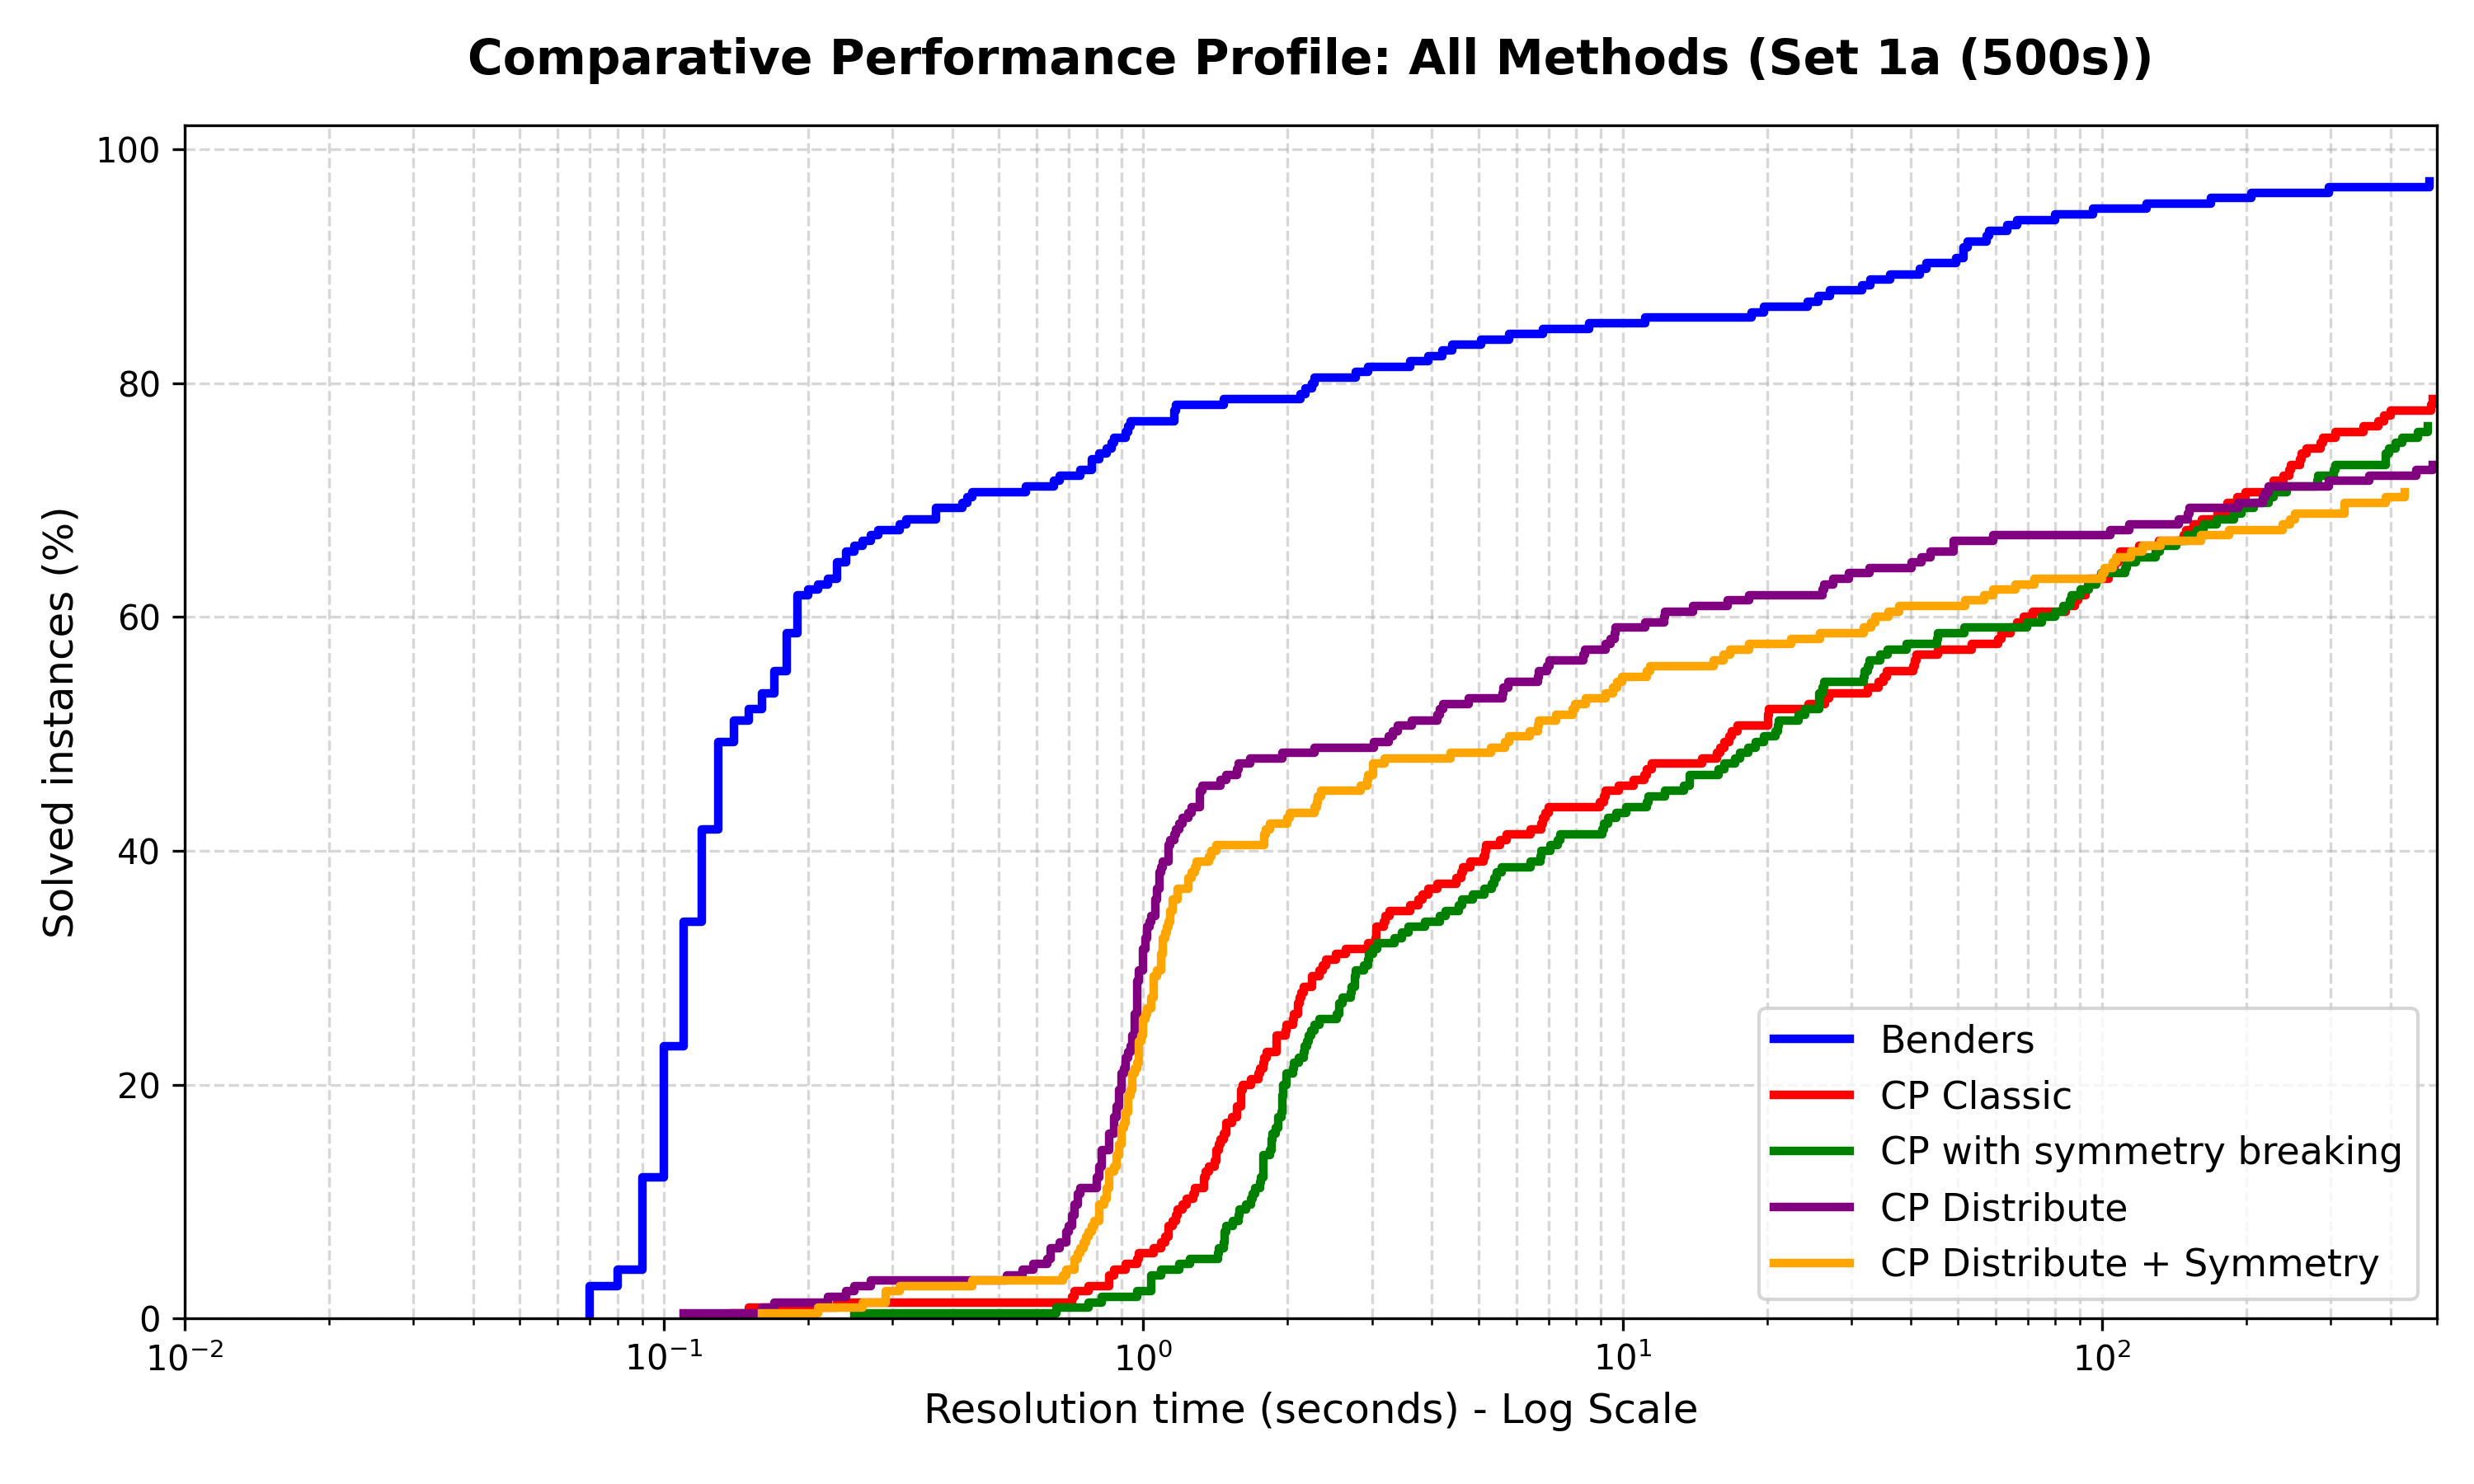
\includegraphics[width=0.85\textwidth]{imports/set1a-profil-performance-complet.png}
    \caption{Profil de performance cumulatif unifié : Comparaison du taux de résolution (\%) en fonction du temps de calcul (échelle logarithmique) sur le Set 1a (215 instances - 500s).}
    \label{fig:profil_perf_set1a}
\end{figure}

\subsubsection{Impact du nombre de travailleurs sur les performances de résolution}

Parmi les différentes caractéristiques structurelles des instances du \texttt{Set 1a}, l'analyse expérimentale révèle que l'effectif de travailleurs $m$ est le facteur qui exerce l'impact le plus déterminant sur les performances de résolution. La figure~\ref{fig:set1a_dataset_analysis_m} illustre l'évolution du temps moyen global de résolution en fonction de $m$ pour l'ensemble des méthodes.

\begin{figure}[H]
    \centering
    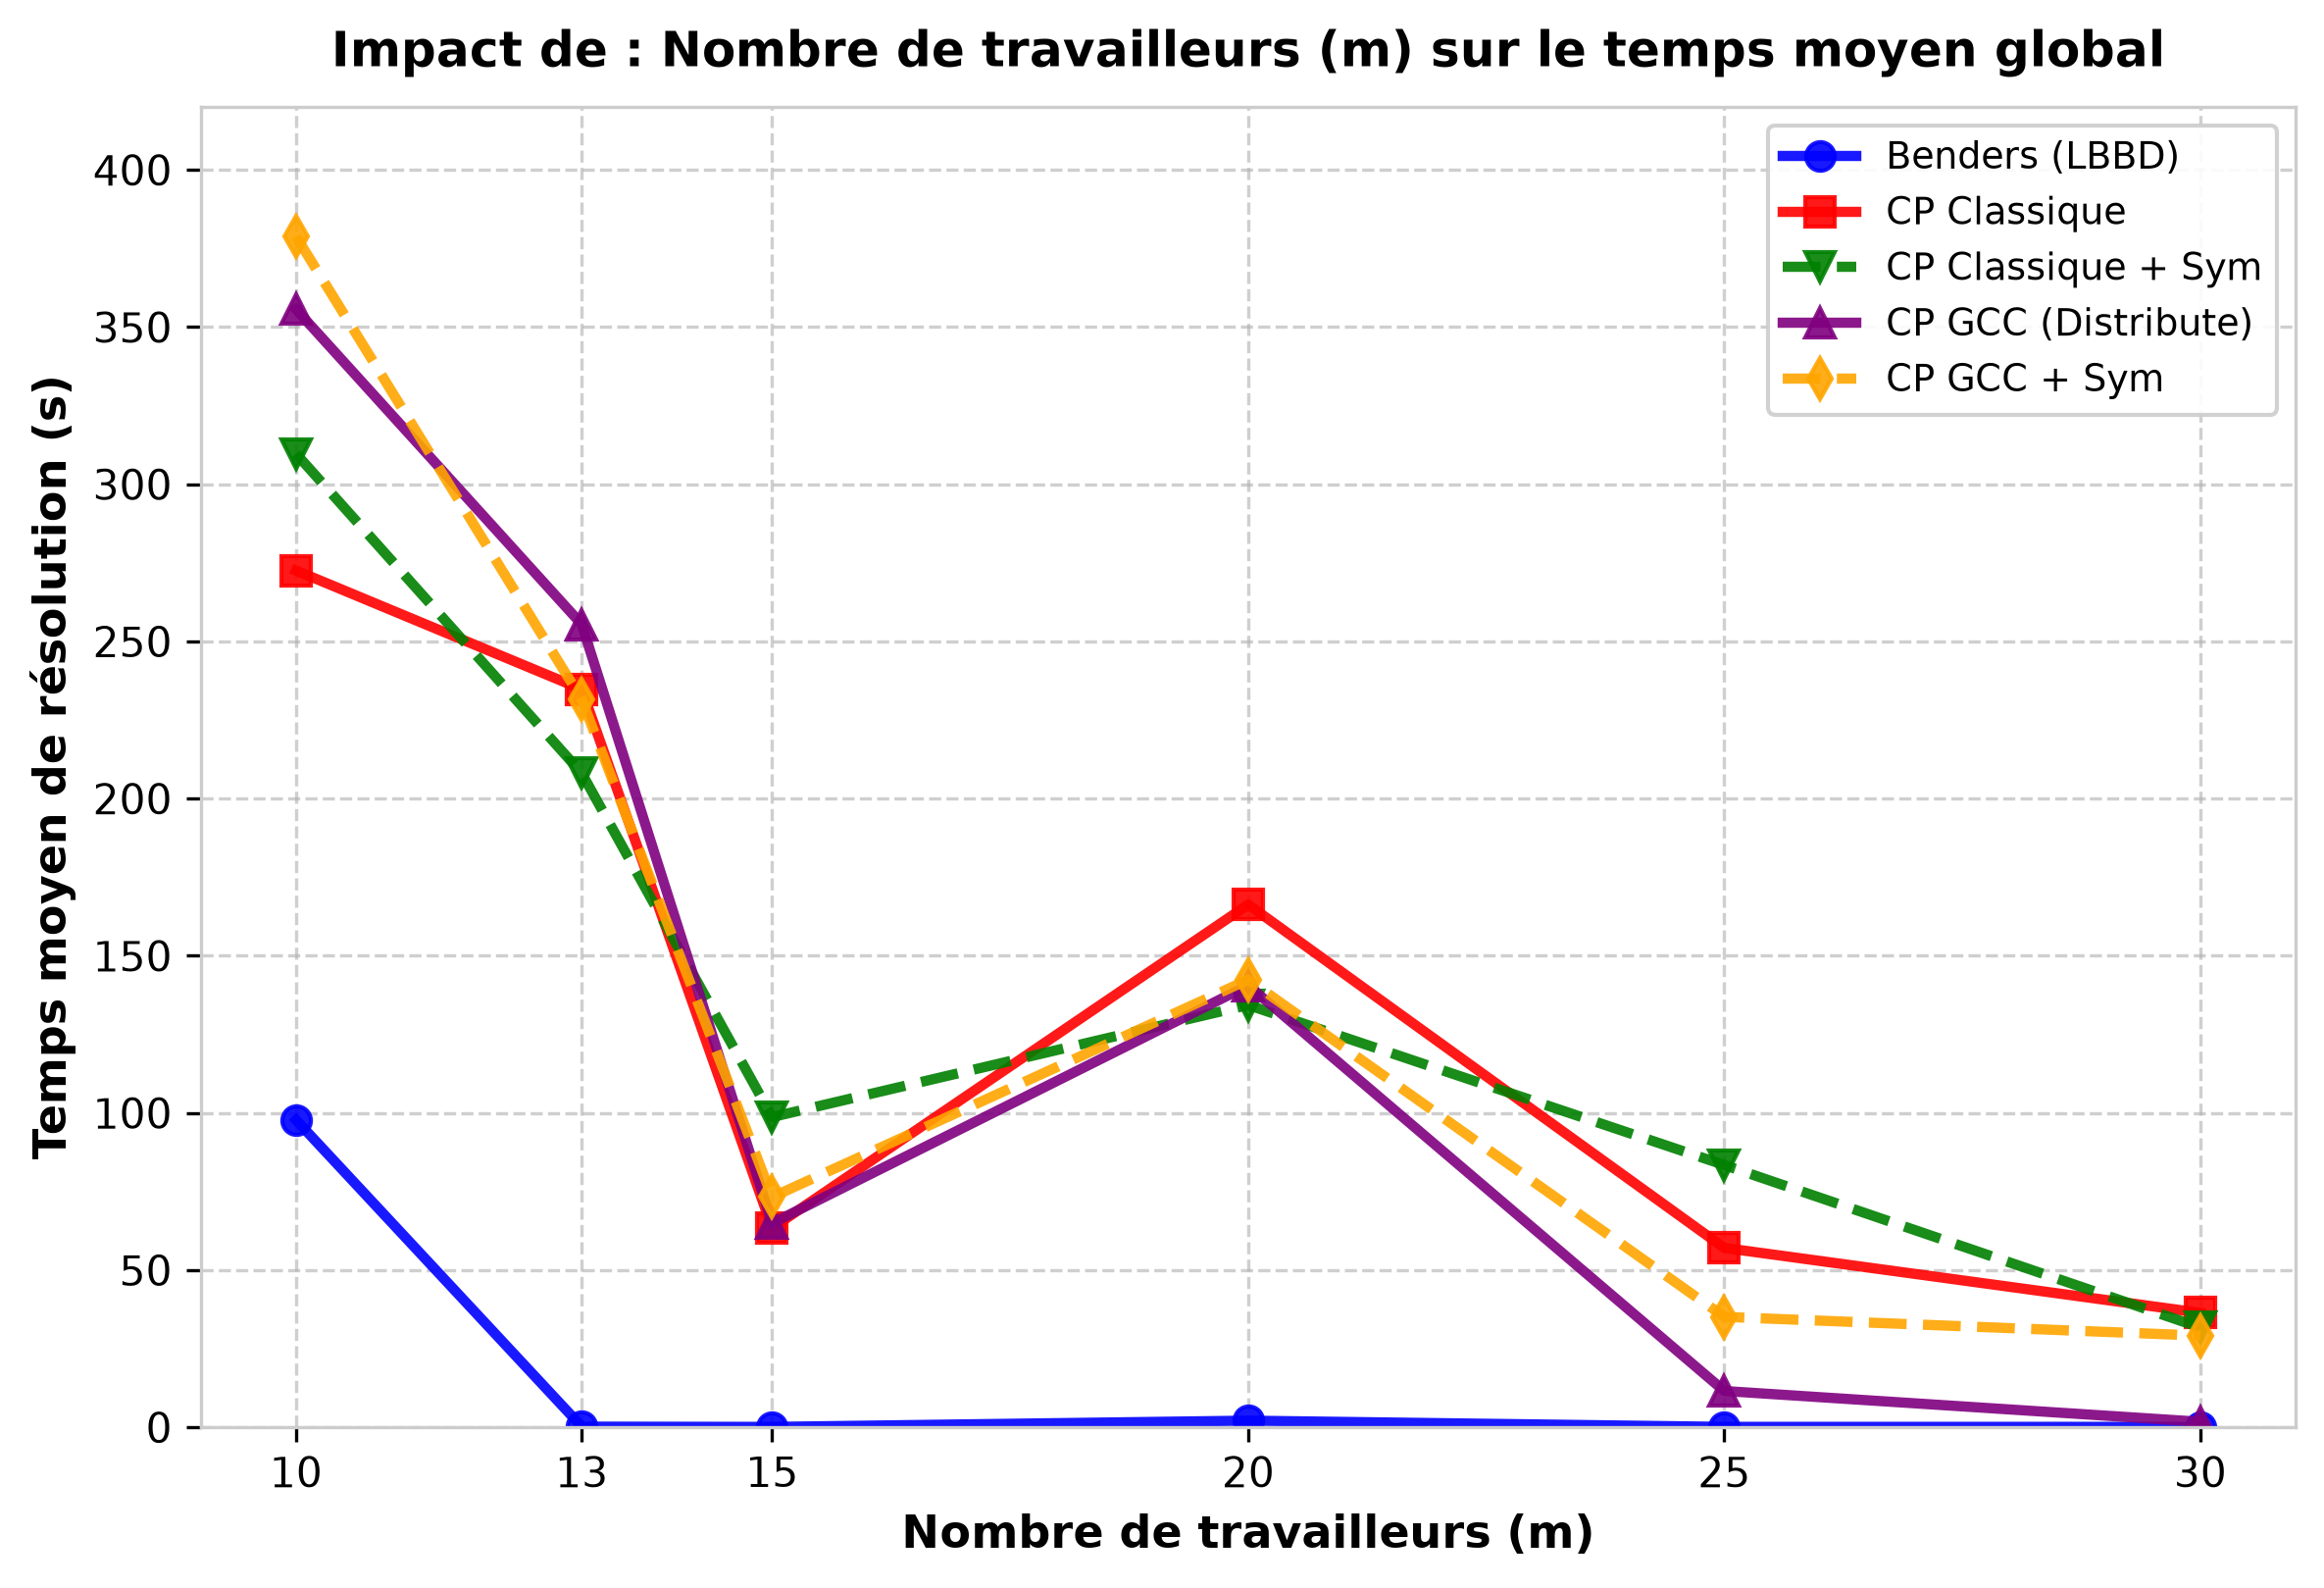
\includegraphics[width=0.85\textwidth]{imports/set1a-dataset-analysis-m.png}
    \caption{Impact du nombre de travailleurs ($m$) sur le temps moyen global de résolution (Set 1a).}
    \label{fig:set1a_dataset_analysis_m}
\end{figure}

On constate de manière très marquée que plus la quantité de ressources multi-compétences augmente, plus les performances s'améliorent. Par exemple, pour la méthode CP GCC, le temps moyen de résolution s'effondre de 378.8 secondes pour $m = 10$ à seulement 1.8 seconde pour $m = 30$.

Sur le plan théorique, la disponibilité d'une main-d'œuvre polyvalente plus nombreuse diminue la rareté des ressources et désature les contraintes d'affectation sur chaque période unitaire. Cela réduit fortement le nombre de conflits d'allocation simultanés et facilite la découverte de plannings réalisables pour le solveur.

\subsection{Résultats et comparaison sur le Subset 1 de MSLIB1}

Les performances de l'ensemble des cinq méthodes de résolution (CP Classique, CP Classique avec bris de symétrie, CP GCC, CP GCC avec bris de symétrie, et LBBD) ont été évaluées sur le sous-ensemble de 200 instances \texttt{Subset 1} de la bibliothèque \texttt{MSLIB1} avec une limite de temps de 500 secondes. Les résultats sont présentés dans le tableau~\ref{tab:results_subset1}.

\begin{table}[H]
    \centering
    \caption{Synthèse globale des résultats de résolution sur MSLIB1 (Subset 1, 200 instances, Time Limit = 500s)}
    \label{tab:results_subset1}
    \small
    \renewcommand{\cellalign}{cc}
    \begin{tabularx}{\textwidth}{|X|c|c|c|c|}
        \hline
        \textbf{Approche} & \makecell{\textbf{Inst.} \\ \textbf{résolues}} & \makecell{\textbf{Succès} \\ \textbf{(\%)}} & \makecell{\textbf{Temps} \\ \textbf{moy. (s)}} & \makecell{\textbf{Temps hors} \\ \textbf{timeouts (s)}} \\ \hline
        \textbf{CP Classique} & 172 / 200 & 86.0\,\% & 78.64 & 10.02 \\ \hline
        \textbf{CP Classique + Symétrie} & 164 / 200 & 82.0\,\% & 100.16 & 12.38 \\ \hline
        \textbf{CP GCC (Distribute)} & 161 / 200 & 80.5\,\% & 105.72 & 10.19 \\ \hline
        \textbf{CP GCC + Symétrie} & 162 / 200 & 81.0\,\% & 102.27 & 8.96 \\ \hline
        \textbf{Décomposition de Benders (LBBD)} & \textbf{188 / 200} & \textbf{94.0\,\%} & \textbf{32.62} & \textbf{2.78} \\ \hline
    \end{tabularx}
\end{table}

\subsubsection{Analyse des taux de résolution et des temps de calcul}
La Décomposition de Benders basée sur la Logique (LBBD) confirme sa supériorité sur ce jeu d'instances plus vaste ($n = 32$ tâches). Elle résout 188 instances sur 200 (94.0\,\%), ne concédant que 12 timeouts. Parmi les instances résolues, 170 l'ont été en moins d'une seconde (90.4\,\%), ce qui illustre la rapidité de la convergence. De plus, la LBBD résout 16 instances qu'aucune méthode CP monolithique n'a pu résoudre, sans qu'aucune instance résolue par le CP ne lui échappe.

\bigskip

Pour les modèles CP monolithiques, le modèle CP Classique résout 172 instances (86.0\,\%), surpassant le modèle CP GCC (161 instances, 80.5\,\%). L'ajout de contraintes de bris de symétrie dégrade les performances du CP Classique (164 résolutions contre 172), mais apporte une légère amélioration sur le CP GCC (162 résolutions contre 161, avec un temps hors timeouts réduit à 8.96\,s).

La LBBD résout l'ensemble des instances en un temps moyen de 2.78 secondes (hors timeouts), avec un nombre d'itérations moyen de seulement {1.23} entre le problème maître et le sous-problème d'affectation (le nombre maximal d'itérations observé étant de 6).

\subsubsection{Comparaison directe sur les instances faciles (communes)}
En isolant les 153 instances résolues à l'optimalité par l'ensemble des cinq méthodes, nous comparons les temps moyens de résolution sans le biais des timeouts :
\begin{itemize}
    \item \textbf{CP Classique :} \textbf{3.22 s}
    \item \textbf{CP Classique avec contrainte de bris de symétrie :} \textbf{6.67 s}
    \item \textbf{CP GCC :} \textbf{9.37 s}
    \item \textbf{CP GCC avec contrainte de bris de symétrie :} \textbf{6.65 s}
    \item \textbf{Décomposition de Benders :} \textbf{0.37 s}
\end{itemize}
Sur ces instances communes, la décomposition de Benders est environ 9 fois plus rapide que le CP Classique (0.37\,s contre 3.22\,s) et 25 fois plus rapide que le CP GCC.

\subsubsection{Comparaison du comportement MSLIB vs Set 1a}
La confrontation des deux jeux de données révèle quatre enseignements principaux :
\begin{enumerate}
    \item \textbf{Le CP Classique est plus rapide hors timeouts sur MSLIB1 :} Le temps moyen hors timeouts chute de 56.38\,s (Set 1a) à 10.02\,s (Subset 1). L'effectif moyen de travailleurs plus élevé ($m \approx 49$) pour un nombre de compétences restreint ($|\mathcal{L}| = 4$) rend l'affectation moins tendue, favorisant la propagation.
    \item \textbf{Écart réduit pour le modèle GCC :} L'avantage du modèle GCC sur les instances faciles s'estompe sur MSLIB1 (10.19\,s contre 10.02\,s pour le CP Classique), car la réduction du nombre de variables d'intervalles apporte moins de bénéfices quand la capacité en ressources n'est pas le facteur le plus restrictif.
    \item \textbf{Sensibilité au bris de symétrie :} Si les contraintes de bris de symétrie dégradent le CP Classique sur les deux jeux, elles deviennent légèrement bénéfiques pour le CP GCC sur MSLIB1 (+1 instance résolue, 8.96\,s contre 10.19\,s), les symétries de permutation étant plus marquées avec des effectifs plus larges.
    \item \textbf{Convergence encore plus rapide pour Benders :} Le nombre moyen d'itérations passe de 1.6 sur le Set 1a à 1.23 sur Subset 1, confirmant que l'efficacité de la coupe minimale ne s'altère pas lorsque le nombre de tâches augmente.
\end{enumerate}

\subsection{Visualisations graphiques pour le Subset 1}
La figure~\ref{fig:profil_perf_subset1} présente le profil de performance cumulatif unifié pour l'ensemble des méthodes sur le \texttt{Subset 1} de MSLIB1.

\begin{figure}[H]
    \centering
    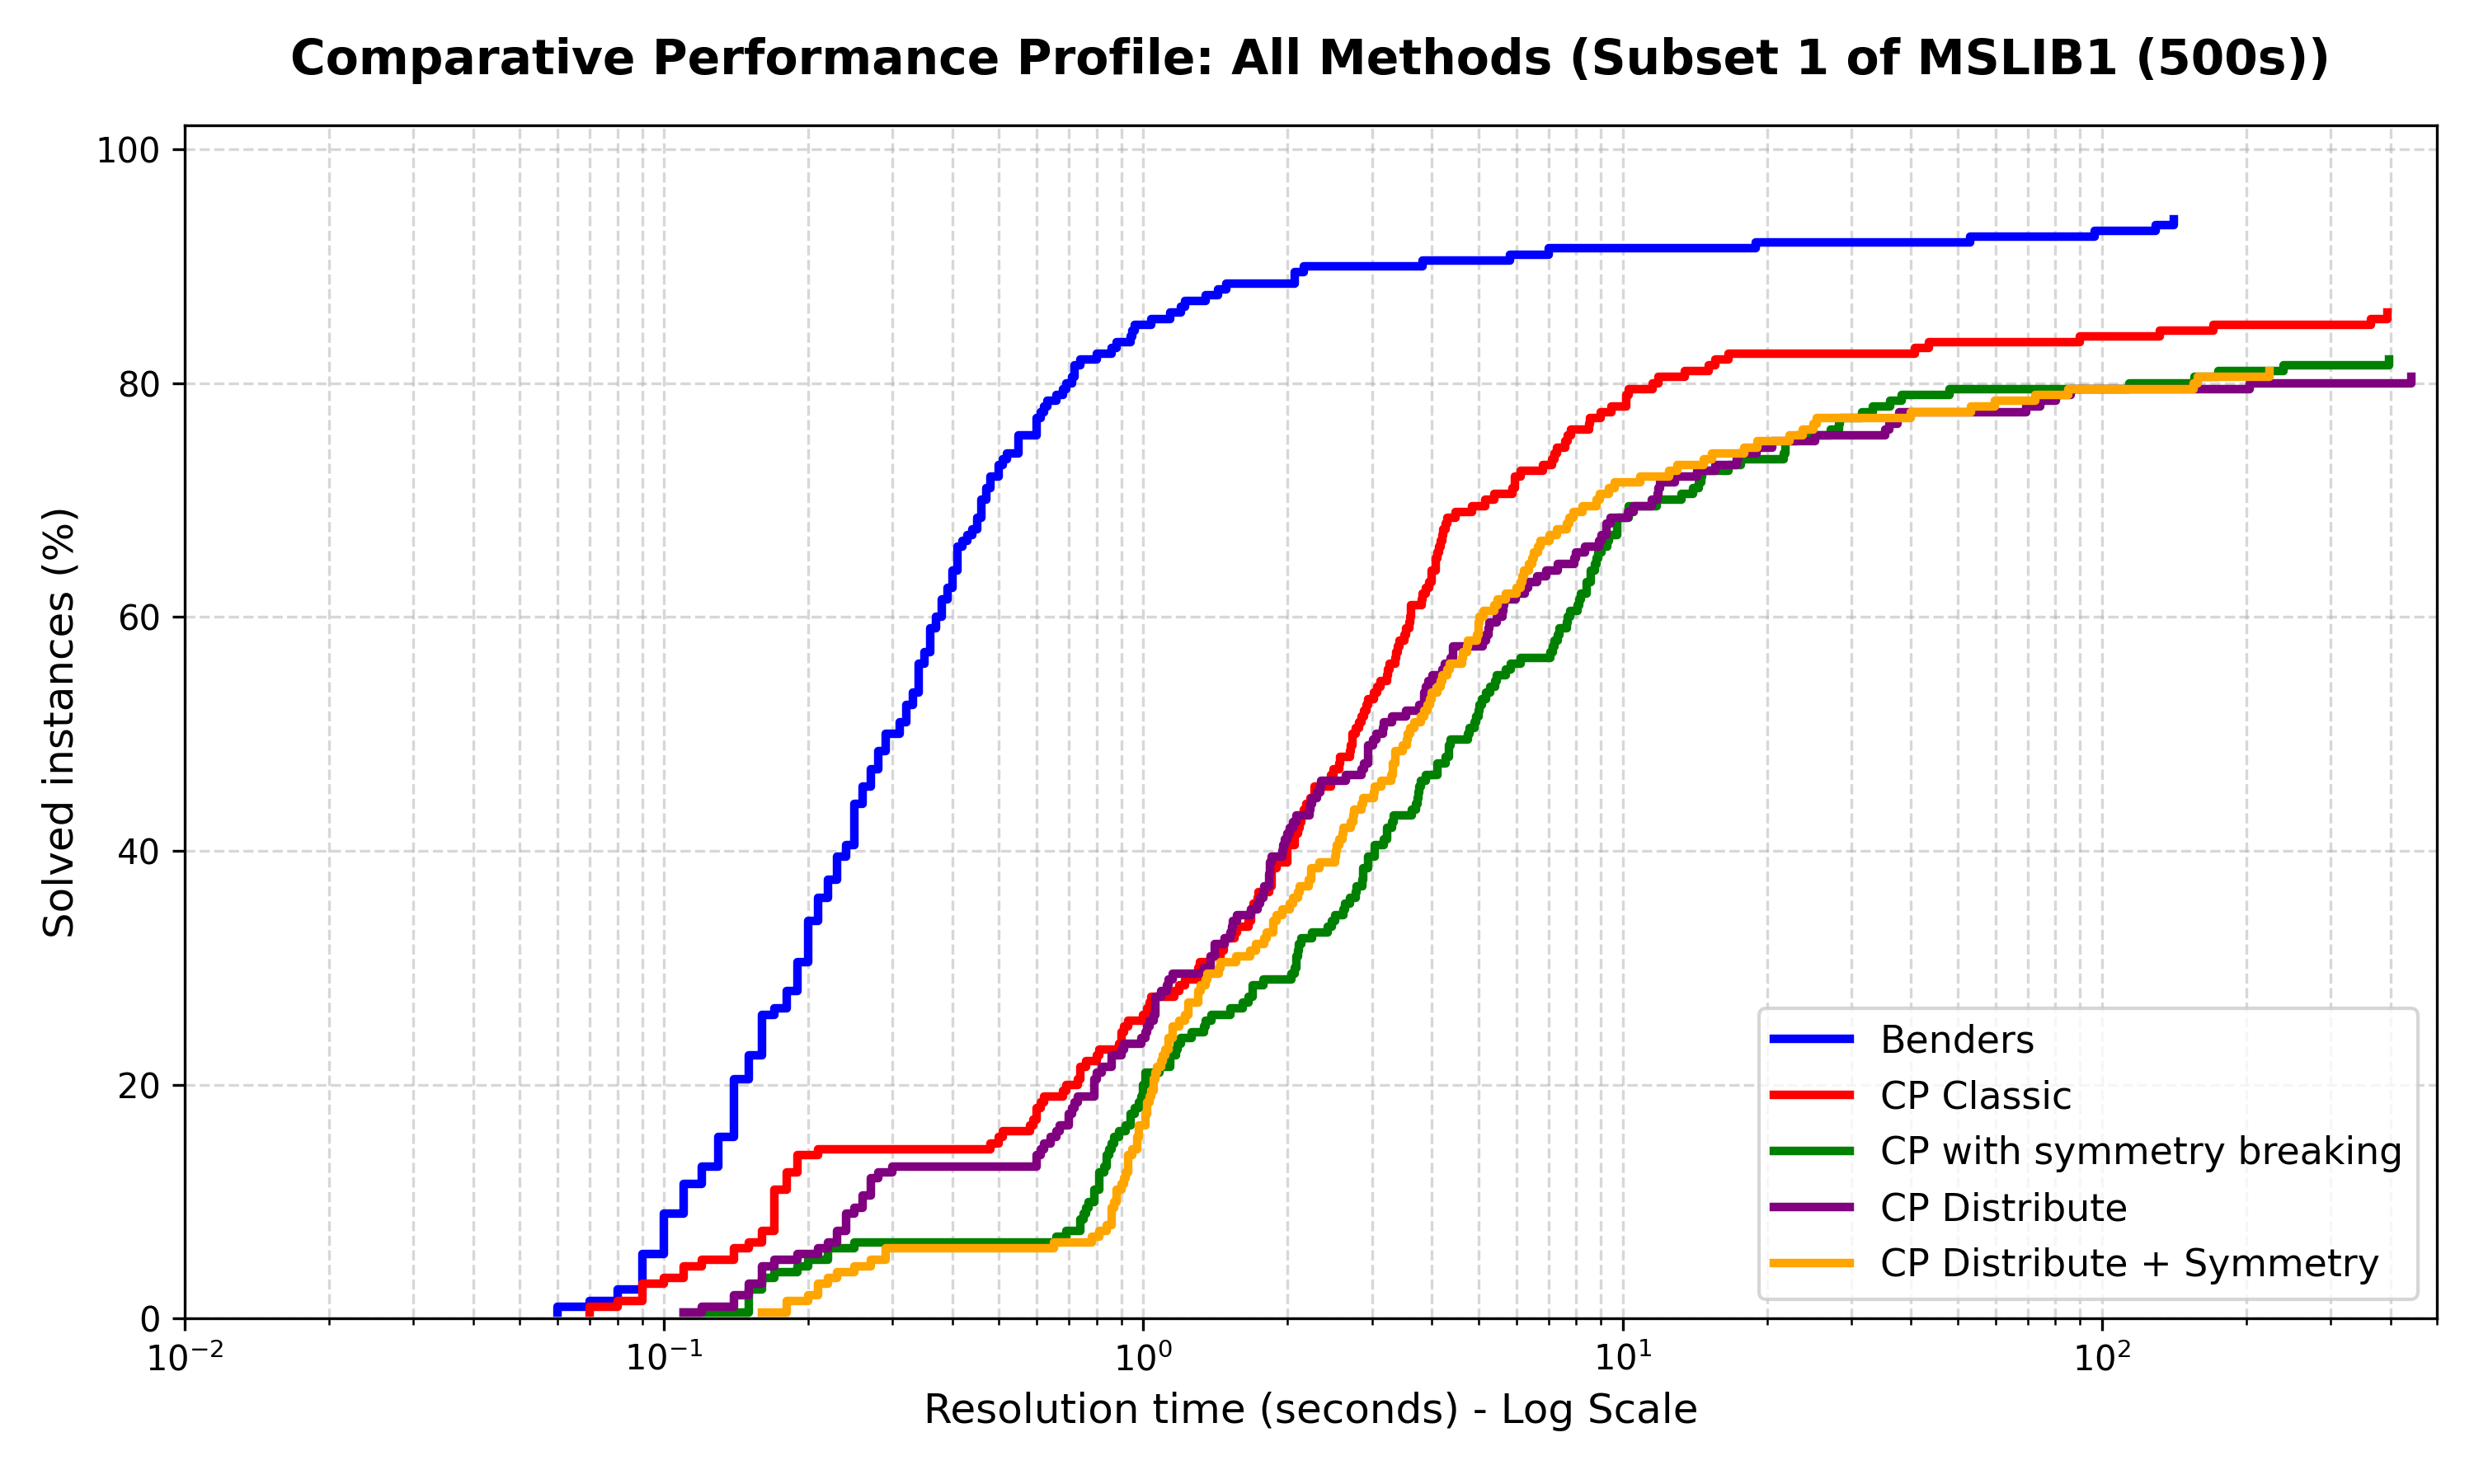
\includegraphics[width=0.85\textwidth]{imports/subset1-profil-performance-complet.png}
    \caption{Profil de performance cumulatif unifié : Comparaison du taux de résolution (\%) en fonction du temps de calcul (échelle logarithmique) sur MSLIB1 (Subset 1 - 200 instances - 500s).}
    \label{fig:profil_perf_subset1}
\end{figure}

